\section{Background Research}
  \citetrackerfalse

  \subsection{What is COVID-19?}
    \par COVID-19 is part of a large family of Coronaviruses which cause respiratory infections. The virus first emerged in December 2019, Wuhan City, China \parencite{HealthGovAU}.
    \par These infections can range from just common cold to more life-threatening diseases such as Middle East Respiratory Syndrome (MERS) and Severe Acute Respiratory Syndrome (SARS) \parencite{Q&A_WHO}.
  
    \par How did COVID-19 come into existence? \parencite{CoronavirusOrigin}
      \begin{itemize}
        \item Evolutionary biologist Jemma Geoghegan of the University of Otago pointed out that the genome of SARS-CoV-2 - the virus which causes COVID-19 - closely resembles those of other viruses already existing in wild animals. 
        \par ``There is a virus in bats, as well as a virus in pangolins, that shares similarities with the new virus that has appeared in humans," said Dr Geoghegan.
        \item Veterinarian and environmental scientist Hume Field from the EcoHealth Alliance stated ``We don't need to manufacture this virus, it exists in nature as it is". 
        \par Dr. Field continued, ``From a scientific point of view, that argument that it's a manufactured virus has been totally discredited".
        \item Despite the fact that many early cases of COVID-19 were related to a live animal market in Wuhan City, we are still incapable of making the claim that this market was the place where the virus made the species barrier jump from some animal to human. 
        \par ``To be honest, I'm not sure if we'll ever know that because the wet market has now been cleared and been decontaminated," Dr Geoghegan said.
        \item As studies have shown that, in terms of genetics, there is a 96 percent similarity between SARS-CoV-2 and a bat coronavirus.
        \par And it is also recorded in the past that both SARS-CoV-1, the virus which caused the SARS outbreak in 2003, and MERS‐CoV, the virus that causes MERS, are found in bats. 
        \par Those facts led Dr. Geoghegan to a conclusion: ``It's likely that this new SARS virus has a similar route, ..."
        \item ``Human interactions with live animals make a host jump more likely to occur," Dr Geoghegan confirmed. And it is clear that the live animal markets are where this kind of interactions happen on a daily basis. 
        \par ``These locations can act as mixing pots, and you can have animals defecating, urinating, they're stressed maybe, you're bringing together the different species that may not be together," infectious disease ecologist David Hayman from Massey University said.
        \par ``And if hand hygiene and stuff like that isn't optimal, then this is where you have the opportunity for an infection to go from one species to another, and that includes humans."
        \par Dr. Field also added that live animal markets are the ideal scenario for host jumping of a virus to happen:
        ``You've got this mixing of species and this potential mixing of viruses in these animals that are under stress, sick and dying as they've gone from their wild environment to the market."
        \item ``If bats are the reservoir hosts of this coronavirus, it probably co-evolved with them over millions of years of their evolutionary history." Dr Geoghegan said.
        \par A recent research Dr. Field mentioned has also discovered that the existence of coronaviruses in bats was dated back to, if not thousands or millions of years, at least 10,000 years.
        \par ``These are very robust and sort of long-term evolutionary relationships of these viruses with these bats," the veterinarian proposed.
      \end{itemize}

  \subsection{How does COVID-19 behave and affect humans?}
    \begin{itemize}
      \item Symptoms: \parencite{HealthGovAU}
        \begin{itemize}
          \item fever
          \item coughing, a sore throat and fatique
          \item shortness of breath
        \end{itemize}
      \item Patients may gradually develop these mild symptoms: aches and pains, nasal congestion, runny nose, sore throat or diarrhea.
      \par Some people may not even know they are infected as they neither experience any previously mentioned symptoms nor feel unwell.
      \par Approximately 80\% of the infected can recover without any kinds of special treatment. Statistically, for every 6 people infected with COVID-19, one becomes seriously ill and develops difficulty breathing. People more probable to be stricken by the virus are the elderly and anyone with historic medical issues such as high blood pressure, cardiovascular diseases or diabetes \parencite{Q&A_WHO}.
      \item The interval of time starting from a person catching the virus until he/she begins to show symptoms is called the ``incubation period", which can range from 1-14 days but most commonly around five days \parencite{Q&A_WHO}.
      \item As suggested by studies and preliminary information on the COVID-19 virus, depending on environmental elements like surface type, temperature or humidity, a few hours or even several days is how long the virus can survive on surfaces \parencite{Q&A_WHO}.
      \item COVID-19 does not disperse in the air as the main way the virus transmits is through droplets, which are already too heavy thus will quickly land on some surfaces, an infected person produces when he/she coughs, sneezes, or speaks.
      \par Nevertheless, these droplets can still float in the air for as far as 1 metre away from the infected person. Therefore, apart from touching contaminated surfaces and then your eyes, nose or mouth later on before washing your hands, being in close contact (within 1 metre) with a person having COVID-19 may also get you infected by breathing in those droplets \parencite{Q&A_WHO}.
      \item For the time being, no vaccine or antiviral medicine has been confirmed 100\% effective in the prevention and treatment of COVID-19.
      \par Since antibiotics only work on bacterial infections, they prove ineffective against COVID-19, which is caused by a virus \parencite{Q&A_WHO}.
      \item Reinfection \parencite{Reinfection_abcnews} \parencite{Reinfection_independent}:
      \par Does your recovery from the virus mean you are safe from it? Many people question whether we can be infected a second time by COVID-19. One such example, in South Korea, there are 91 cases tested positive again after testing negative. Jeong Eun-kyeong, director of the Korea Centers for Disease Control and Prevention, said that it might be the virus that is reactivated not the patients being reinfected. Some cases that tested negative one day and positive another day during hospitalization. This is a complicated problem because if the result of tests is wrong, we might discharge patients who are still carrying the virus. Scientists and doctors are still working on the data from those cases to learn more about the behaviors and characteristics of this virus.
      \par According to a study in Shanghai, approximately one-third of the tested patients develop poor levels of antibodies. Lack of antibodies being produced also means a lack of immunity. There is an idea to use antibody testing to find out who is immune to the virus and who is not. However, Mary Carol Jennings, a physician and vaccine scientist, said “the logistics of making tests widely and fairly available are fraught, and we shouldn't pin our hopes to a single strategy.” Donald Trump,President of the USA, also said that he wanted everyone to be tested by this tool before the country operates normally again.
      \par Although coronaviruses have existed for a while and we have certain knowledge about them, scientists are still not sure about the immune response to this coronavirus. They need more time to do experiments on blood samples from cases around the world before going into a conclusion. ``COVID-19 has emerged so recently, we know very little about whether or not an initial infection 'teaches' the immune system how to protect against a future infection," explained Mary Carol Jennings.
    \end{itemize}
  
    \subsection{How does COVID-19 spread?}
      \par According to \textcite{Q&A_WHO}, all of the followings are possible trasnmission routes of COVID-19:
      \begin{itemize}
        \item This disease spreads from infected patients to others whom they have been in contact with even during the incubation period.
        \item The virus spreads through droplets from the nose or mouth of the infected person when he/she coughs, sneezes or exhales.
        \item People may be infected by breathing in droplets from the one that they are talking to and this is the main reason why social distancing is important. The safe distance between is about 1 meter away from the infected person.
        \item This coronavirus can last on surfaces and objects (namely tables, chairs, elevator buttons, etc.) for hours or up to days. Consequently, people can get infected by touching these objects which contain the virus and then touch their eyes, nose or lips.
        \item Although the rate of catching this virus from the one that has no symptoms is modest, people still need to be extremely careful when approaching someone. The reason is that at the initial stages of the disease, there are some patients who just show very mild symptoms like coughing and they do not notice that they may be infected until these symptoms become more severe.
        \item Despite the fact that the virus may exist in feces from the infected person, the proportion of spreading through this way is negligible. All you need to do is washing hands before meals and after using the toilet.
      \end{itemize}

    \subsection{Precaution and Prevention}
      \par To help suppress and possibly eradicate this new devastating virus COVID-19, \textcite{Q&A_WHO} encourages all individuals to practice the following hygiene/safety habits:
      \begin{itemize}
        \item Wash your hands after returning home and before entering your workplace or public places. You can clean your hands with hand sanitizer or with normal soap and water.
        \item Keep the distance about 1 meter from others in public to not only protect yourself but also the community.
        \item Minimize as much as possible touching your face, eyes and nose.
        \item Make sure that your family members or whoever living with you practice good hygiene. Remember to cover your mouth and nose whenever you cough or sneeze so that your droplets cannot land on public items.
        \item Please self-quarantine if you feel sick. If you experiencing symptoms like shortness of breath, fever or cough, contact your local health department and follow their instructions.
      \end{itemize}

    \subsection{Existing Pandemic-countering Measures/Technologies}
      \begin{itemize}
        \item How China slows down the virus \parencite{ChinasMeasure1} \parencite{ChinasMeasure2}:
        \par The Chinese government is very strict in monitoring their people in public places. There are CCTVs everywhere with face recognition technology integrated to find out who is not wearing a facemask or detect who has high hypothermia. Whenever people enter a building or workplace, they must declare their personal information, scan the QR code and write down their travel history in the last few days. A few residents said that they feared the surveillance would continue after the pandemic outbreak had been stopped. Every time they go out, they always feel like being stalked by somebody.
        \par One of the reasons that China has done so well in stopping the pandemic is mass quarantine. The government turns large places such as stadiums and hotels into quarantine centers to prevent the virus from spreading to the community. Moreover, many hospitals, which mainly focus on COVID19-infected patients, have been constructed. Many ways of penalty and reward have been proposed by the government to make sure that their people follow social distancing regulations. China virus tracking teams are surprisingly responsive despite dense population. They quickly isolate the infected patient as soon as possible and their friends, family members or roommates.

        \item BlueDot \parencite{BlueDotHome} \parencite{BlueDotCNBC}:
        \par BlueDot is a proprietary software-as-a-service designed to track, locate and conceptualize infectious disease spread. It warns health care, government, business, and public health clients about a summary of an abnormal epidemic disease that its Artificial Intelligence has identified and the hazards it may pose. Big data plays a pivotal role in crawling data from hundreds of thousands of sources, including statements from official public health organizations, digital media, global airline ticketing data, livestock health reports and population demographics by using natural language processing and machine learning. It’s capable of swiftly analyzing extensive information every 15 minutes, 24 hours a day.
        \par Moreover, not only is Blue Dot discovering epidemic disease as soon as possible, but it can also understand how diseases might disperse all over the world, and then identify the potential consequences it might lead to. Furthermore, by collecting global airline ticketing data, BlueDot was also able to precisely determine the places which would have the highest volume of travelers from Wuhan, including Bangkok, Hong Kong, Tokyo, Taipei, Phuket, Seoul, and Singapore. As a result, the top 11 cities of their list were considered to be first places to be infected with COVID-19.
        \par Blue Dot was founded by Kamran Khan - an epidemiologist and physician, who is self-described as an “accidental entrepreneur”. The severe acute respiratory syndrome (SARS) outbreak in 2003 deeply motivated him to start the project and find better solutions for infectious disease threats in the future.

        \item Contact Tracing:
        \begin{itemize}
          \item What is Contact Tracing?
          \par Against such a novel and highly-infectious virus like Covid-19, as we do not yet have the vaccine, contact tracing is one of the most effective weapons. According to the website of Queensland Health \parencite{QueenslandHealth}:
          \par ``Contact tracing is a process used to understand how an infectious disease is spreading in a community. Contact tracing has two purposes: to figure out who a sick person caught an illness from, and to find out who they’ve been in contact with while infectious.".

          \item Singapore's TraceTogether, Israel's TheShield and a contact tracing system Apple and Google are currently working on:
          \par Some mobile applications with similar purposes have been put into use in some countries, namely ``TheShield" in Israel \parencite{IsraelTheShield} and ``TraceTogether" \parencite{SingTraceTogether} in Singapore. For ``TheShield", the app takes location data of the user and compares that to the locations of confirmed cases to check if the user is at risk of being infected. If the app confirms that the user is indeed at risk, the user can choose to report themselves to the health authorities after filling out a form. On the other hand, ``TraceTogether" uses a different approach to contact tracing. Rather than taking users' location data, the app utilizes a Bluetooth protocol that allows nearby phones in an area exchange signals with each other. Each phone will then remember other phones that it has exchanged signals with in the last 21 days. In addition, location data is not collected. Compared to the ``centralized" approach of ``TheShield", where all the data is stored in one database of the authorities, this ``decentralized" approach partly helps deal with the concern of user's privacy. Recently, a similar system to ``TraceTogether" has been proposed and under-developed by Apple and Google, where the location data will not be collected \parencite{AppleGoogleSys}. Having said that, this decentralized approach is also not perfect, especially when there have been evidences that Covid-19 does not only transmit through direct contact.

          \item MIT-developed app system that uses Bluetooth signals to aid contact tracing while preserving privacy \parencite{MIT_App}:
          \par “Find My \parencite{AppleFindMy} inspired this system. If my phone is lost, it can start broadcasting a Bluetooth signal that’s just a random number; it’s like being in the middle of the ocean and waving a light. If someone walks by with Bluetooth enabled, their phone doesn’t know anything about me; it will just tell Apple, ‘Hey, I saw this light,’” says Marc Zissman, the Associate Division Head at MIT Lincoln Laboratory and co-principal investigator of the project.
          \par The project is fundamentally expecting a smartphone to constantly transmit and keep a log of contingent signals using their system. Simultaneously, the smartphone traces chirps found from other devices and only logs vigorously considerable chirps for contact tracing — those radiated from within 1.83 meters and acquired for a precise period.
          \par Users would participate by downloading an application that supports this tool. After a COVID-19 diagnosis, those people would be given a QR code from a health agency. They can also transfer their log to the digital computer data storage by scanning this QR code. These logs could be scanned by everyone using the app through their smartphones. A warning could notify a phone owner of the estimated distance to an active case if the system found a match.
          \par “We’re not tracking location, not using GPS, not attaching your personal ID or phone number to any of these random numbers your phone is emitting,” says Daniel Weitzner, a principal research scientist in the MIT Computer Science and Artificial Intelligence Laboratory (CSAIL) and coprincipal investigator of this effort. “What we want is to enable everyone to participate in a shared process of seeing if you might have been in contact, without revealing, or forcing anyone to reveal, anything.”
          \par The selection is optional. Weitzner guarantees that the app would respect the civil and human rights to not use the tool. The best thing we can do is expect that the populace would cooperate with the project to slow down the COVID-19 outbreak. “We need a large percentage of the population to opt in for this system to really work. We care about every single Bluetooth device out there; it’s really critical to make this a whole ecosystem,” he said.  
        \end{itemize}

        \item Discussion on these measures/technologies:
        \begin{itemize}
          \item The mass population surveillance and forced quarantine approach taken by China and South Korea has proved highly effective in the situation of escalating infection rate witnessed in these two countries. Nevertheless, such pandemic control method fails to guarantee the rights of privacy for the Chinese and Korean citizens. Therefore, in nations where the state of viral infection is not too severe, alternative measures apart from that currently adopted by China and South Korea will be extensively more desirable.
          \item With respect to global pandemic prediction and monitoring, BlueDot is unquestionably the right tool for the job, but that is also as far as BlueDot can go. Where BlueDot succeeds in offering globally applicable pandemic-countering measures, it is, on the other hand, unable to effectively tackle the precise level of each and every individual. We can understand the incapability of BlueDot simply by just considering how massive the amount of data it is already processes at the moment to be able to achieve what it is doing, hence monitoring at individual level would introduce unimaginable loads of data to be handled. Moreover, directing personal data around the globe into the hand of a single organization definitely will make privacy concerns and ethical issues turn to an even worse path. That is why we are still calling for an accurate, individual-level control method and thus, contact tracing.
          \item Except for Israel's ``The Shield'' which requires users' location data to function, all other contact tracing mobile applications aforementioned such as ``TraceTogether'' by Singapore, the two systems developed by Google, Apple and MIT University and specifically to Australia - the ``COVIDSafe'' app \parencite{CovidSafe} - utilize only the Bluetooth communication technology and avoid the usage of GPS services or any kind of location data for that matter to assure users with privacy preservation. However, not only is COVID-19 known to transmit through close-quarter contacts, it can also survive on object surfaces for a long period of time, thus also infecting anyone who touches these surfaces. Not exploiting location data secures users' privacy to some extent yet at the cost of not being able to trace back highly infectious locations. Acknowledging this fact, our app aims to mitigate as many as possible the issues posed by or experienced in other approaches and exactly how we plan to do that will be presented shortly in next sections.
        \end{itemize}
      \end{itemize}

  \subsection{Privacy Concerns}
    \subsubsection{User Concern}
      \par High possibility of exposing the location shared by the user (IP Leak) to the any kind of data breaches that may disclose the information towards unauthorized outsiders. Most cases were happened with an unguarded architecture through connection (e.g. database) or information without implementing encryption technology \parencite{Ian1}. According to \textcite{Ian2}, various companies sell, use or analyse the data to cater their clients through studying consumer behaviour, which prompted users to share their location without providing disclosure of the privacy policy with clarity upon the data collected. A study shown that users are also worried of the location tracking could put their close ones at risk through studying their routine, making their closed ones vulnerable to crimes \parencite{Ian3}.

    \subsubsection{National Establishment}
      \par There is no universal data protection and privacy law to be complied by all the registered countries by far. It has been stated in \textcite{Ian4} that the respective country law is being complied whenever the data is transmitted between countries. Hence, the enaction of a universal privacy and protection law for all nations to comply would be a sophisticated process. However, large regional union (e.g. European Union) had established a regulation called General Data Protection Regulation (GDPR) which all EU countries are to pass this law on federal level for data collection and processing. This is a huge milestone for regional unions of countries with diplomatic collaborations to enact laws on a higher level for legislations.
      \par An online journal of European Union \parencite{Ian5} concludes that the GDPR regulation emphasize on the fundamental rights and freedoms of natural persons with regards to the processing and movement of data should be adhered to all legal rules set for the protection of natural persons.

    \subsubsection{Australian Law}
      \par Office of Australian Information Commissioner (OAIC) \parencite{Ian6} has provided how GDPR comply with Australian privacy laws. As Australia Privacy Act 1988 (APP) indicated that Section 14 of the Act namely Privacy Principles (IPPs) adopts various transparent information handling practices, Australia and EU countries are compliant with both regulations of GDPR and APP whenever information is made across borders (as mentioned above in National Establishment). As both regulations enacted have different governance structures and preservation upon human rights. I will list the notable differences in information handling practices between both regulations.

\begin{table}[H]
  \begin{tabular}{|p{5cm}|p{5cm}|p{5cm}|}
    \hline
                                  & GDPR                                                                                                                                                & APP                                                                                                                                                                     \\
    \hline
  Compliance                     & \begin{tabular}[c]{@{}p{5cm}@{}} \tabitem Enterprise that have an establishment in the EU\\ \tabitem Enterprise that offers goods or services outside EU\end{tabular} & \begin{tabular}[c]{@{}p{5cm}@{}}\tabitem Australian Government Agencies\\ \tabitem Private Sectors and NGO\\ \tabitem Health Service Providers\\ \tabitem Small Medium Enterprise (SME)\end{tabular} \\
  \hline
  Types of Regulated Information & \begin{tabular}[c]{@{}p{5cm}@{}}\tabitem Collection of specific personal data (e.g. name, location data)\\ \tabitem Web cookies, routine data\end{tabular}           & \tabitem Collection of non-specific personal data that is reasonably identifiable (e.g. social circle)                                                                        \\
    \hline
  Consent                        & \tabitem Freely given, specific and informed with clear indication of written demonstration                                                               & \tabitem Express consent in written demonstration or implied consent through non-verbal communication                                                                         \\
  \hline
  Data Breach Notifications      & \tabitem A 72-hour timeframe to notify involved individuals and relevant authorities                                                                      & \tabitem Notify OIAC as soon as possible \\
  \hline
  \end{tabular}
  \end{table}

      \par In short, GDPR only applied to entities on enterprise level while APP on federal level. Next, GDPR
      will regulates information which includes personal activity data while APP considers data that could
      can be identifiable upon individuals such as social circle and household relationships. Furthermore,
      GDPR and APP both provides express consent for collecting data however APP allows entities to
      collect data upon implied consent as well, which may be unwilling under certain circumstances.
      Moreover, GPDR will allows a timeframe to be given for the entities to notify involved stakeholders
      upon data breaches whereas APP needs to notify the government agencies in an urgent manner.
    
    \subsubsection{Possible Alternatives}
      \begin{enumerate}[a)]
        \item \textbf{Cryptography}
          \par Asymmetric encryption could be a good option in enhancing data security level. Taking the proposing pandemic tracking app as an example, all users will have a public key to encrypt information sent to the application. On the other hand, the government as the application owners should hold the private key to decrypt the information only. \textcite{Ian7} written about a rotation mechanism that Apple uses to change the public key of a feature randomly from time to time, which increase the difficulties for anyone to track the users through location services (e.g. GPS, Bluetooth, hotspot, etc.). Hence, cryptography could be a useful implication to further support data security.
        \item \textbf{Union Law}
          \par As digital users have greatly increased during the recent decades, more people are able to obtain digital devices, such as smartphone for various purposes. In addition, the user community is expanding on a large scale across the globe, data is inevitably channelling across borders and regions, which is necessary for countries to establish unions that can collaborate for handling and exchanging these information (e.g. United Nation). Following data protection and privacy law, it is crucial that a universal law could be listed on legislations for all countries to comply with, that creates a standard of legal rules to protect the fundamental rights of a natural person.
      \end{enumerate}

  \subsection{User Research}
  \begin{enumerate}[1.]
    \item \textbf{Surveys}
      \par Survey is a method of quantitative research. It is used as an approach for collecting a more structured and statistical data for general background study. The participants were from various age groups as there is no conditional user restrictions, the possible solution is to cater all age groups.  Thus, collected responses are used for further evaluation to create a solution for general users. Moreover, this is a crucial process to understand the requirements for system visualization during design planning. The survey was designed through Google Form and made available online. The responses are attached below in Appendix \ref{appendix:quantitative}.
      \par \textbf{Findings}
        \begin{figure}[H]
          \centering
          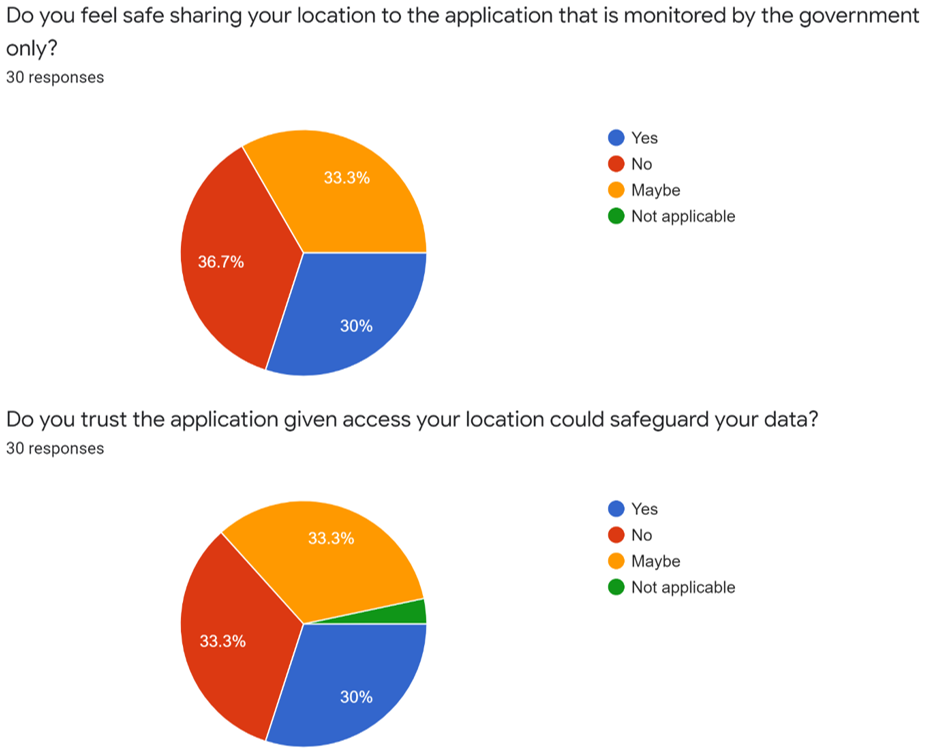
\includegraphics[width=14cm]{quantitative-01.png}
          \caption{}
          \label{fig:quantitative-01}
        \end{figure}
        \begin{figure}[H]
          \centering
          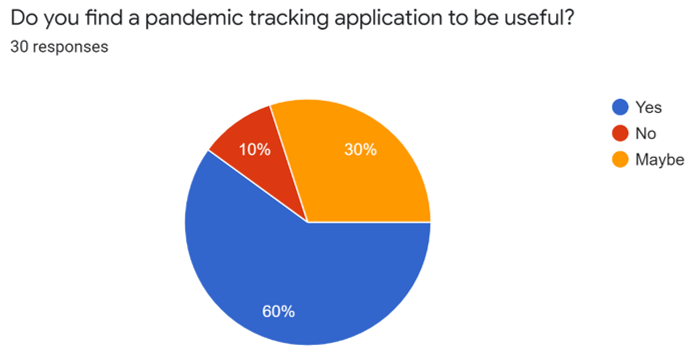
\includegraphics[width=12cm]{quantitative-02.png}
          \caption{}
          \label{fig:quantitative-02}
        \end{figure}
        \begin{figure}[H]
          \centering
          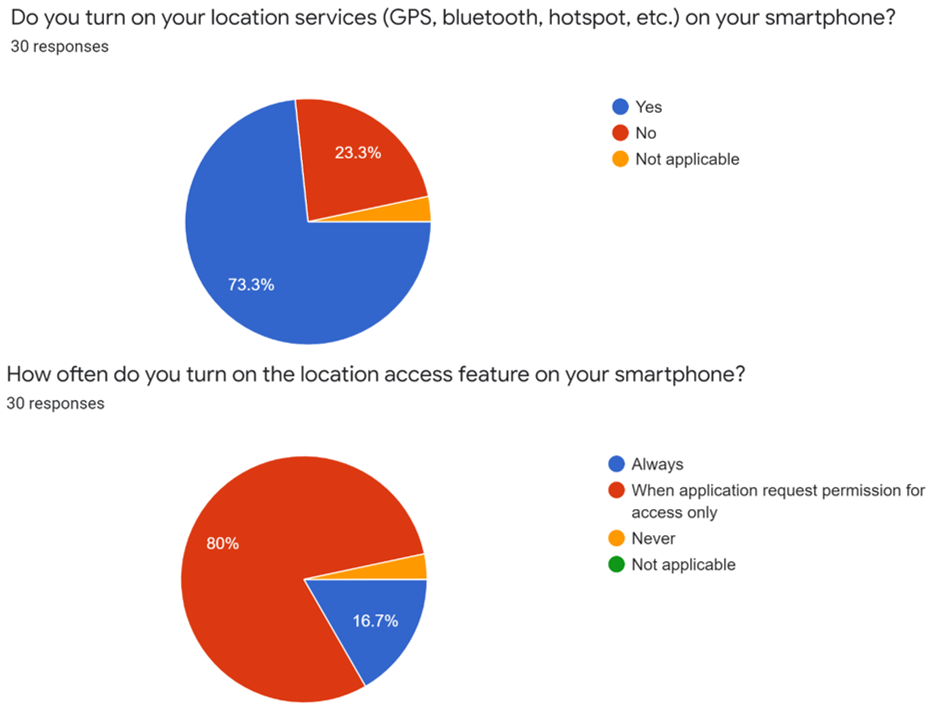
\includegraphics[width=14cm]{quantitative-03.png}
          \caption{}
          \label{fig:quantitative-03}
        \end{figure}

        \begin{itemize}
          \item Based on Figure \ref{fig:quantitative-01}, one-third of the respondents do not trust the data being protected regardless of it being a third-party or the government.
          \item Based on Figure \ref{fig:quantitative-02}, 60\% of the respondents thinks that a contact-tracing application would be useful.
          \item Based on Figure \ref{fig:quantitative-03}, approximately 73\% of the respondents turn on the location service feature which around 80\% gives location access only when the application request from the users.
        \end{itemize}
    \item \textbf{Interviews}
      \par Interview is a method of qualitative research. It is used as an approach for collecting descriptive opinions and views among different specific user categories. The interviewees were focused upon 3 different age groups consists of a primary school student, a retail worker, and a retired elderly that represents the age ranges of 0 to 17, 18 to 64, and above 65 respectively. The interview is composed of designed questions based on the evaluation from the survey, follow-up questions may also be included to gather more in-depth data. Thus, this helps to discover information based on their thinking, attitudes and even motivations. All interviewees have expressed consent to participate in this research study. The interviews were all conducted through online video call. The transcripts are attached below in Appendix \ref{appendix:qualitative}.
      \par \textbf{Findings}
        \begin{itemize}
          \item Minors do not think the application is necessary for them.
          \item Most adults are concern of the user privacy with location sharing.
          \item Includes accessibility features to accommodate elderly with disabilities.
        \end{itemize}
    \item \textbf{Insights}
      \begin{itemize}
        \item The number of application users could directly be influenced with the habit of users utilizing the location services or not, as it is necessary for the application to use the location services feature.
        \item Most participants do not trust the application to always collecting their location data.
        \item Most participants are doubtful of the government credibility in protecting their data. 
        \item Parental guidance and control could be a reason for minors not finding the application useful.
        \item Increasing accessibility features for accommodating user groups with disability could create a higher acceptance among the community.
        \item Proper digital privacy establishment is necessary for users to trust the application provider in handling their data.
      \end{itemize}
  \end{enumerate}

\subsection{What our app tries to achieve}
  \subsubsection{Contact Tracing}
  \par Same as many other existing COVID-19 contract tracing apps, our app will also utilize Bluetooth for close contact logging as this is the best technology we have got for the purpose. As for location logging, our team has considered the scenerio of still collecting location data using GPS services yet letting the users have the choice to opt out the functionality entiredly in case they have any privacy concerns. Based on the user research data displayed above, however, it was soon proven that the majority of users will feel reluctant, even resistive in some occasions, to the idea of live location tracking.
  \par To be able to still record location data and at the same time make the users feel somewhat comfortable with such function, our team has come up with a model that will be beneficial to all of the three important stakeholders - the government, the businesses and the users - as long as each of them agrees to take up certain responsibilities:
  \begin{itemize}
    \item What each stakeholder wants:
      \begin{itemize}
        \item The government: minimizing the number of COVID-19 cases as well as keeping the economy alive, hence complete lockdowns are not desirable.
        \item The businesses: staying open to make money.
        \item The users: being able to freely travel outside yet not risking being infected with COVID-19.
      \end{itemize}
    \item The solution:
      \begin{itemize}
        \item Avoid going into lockdown as much as possible. Consider it as the last resort only.
        \item The government enforces on businesses which wish to stay publicly open a law: businesses must log each and every customer who has visited their place. This can be done via QR codes given from the government to these businesses.
        \item Users must use our app to scan the QR codes of places they want to visit. Businesses have the right to ask and check if their customers have scanned the code. 
        \item As for places without closure like parks, squares, etc. the government can choose to close them up entirely.
      \end{itemize}
  \end{itemize}
  \par The following image summarizes our model:

  \begin{figure}[H]
    \centering
    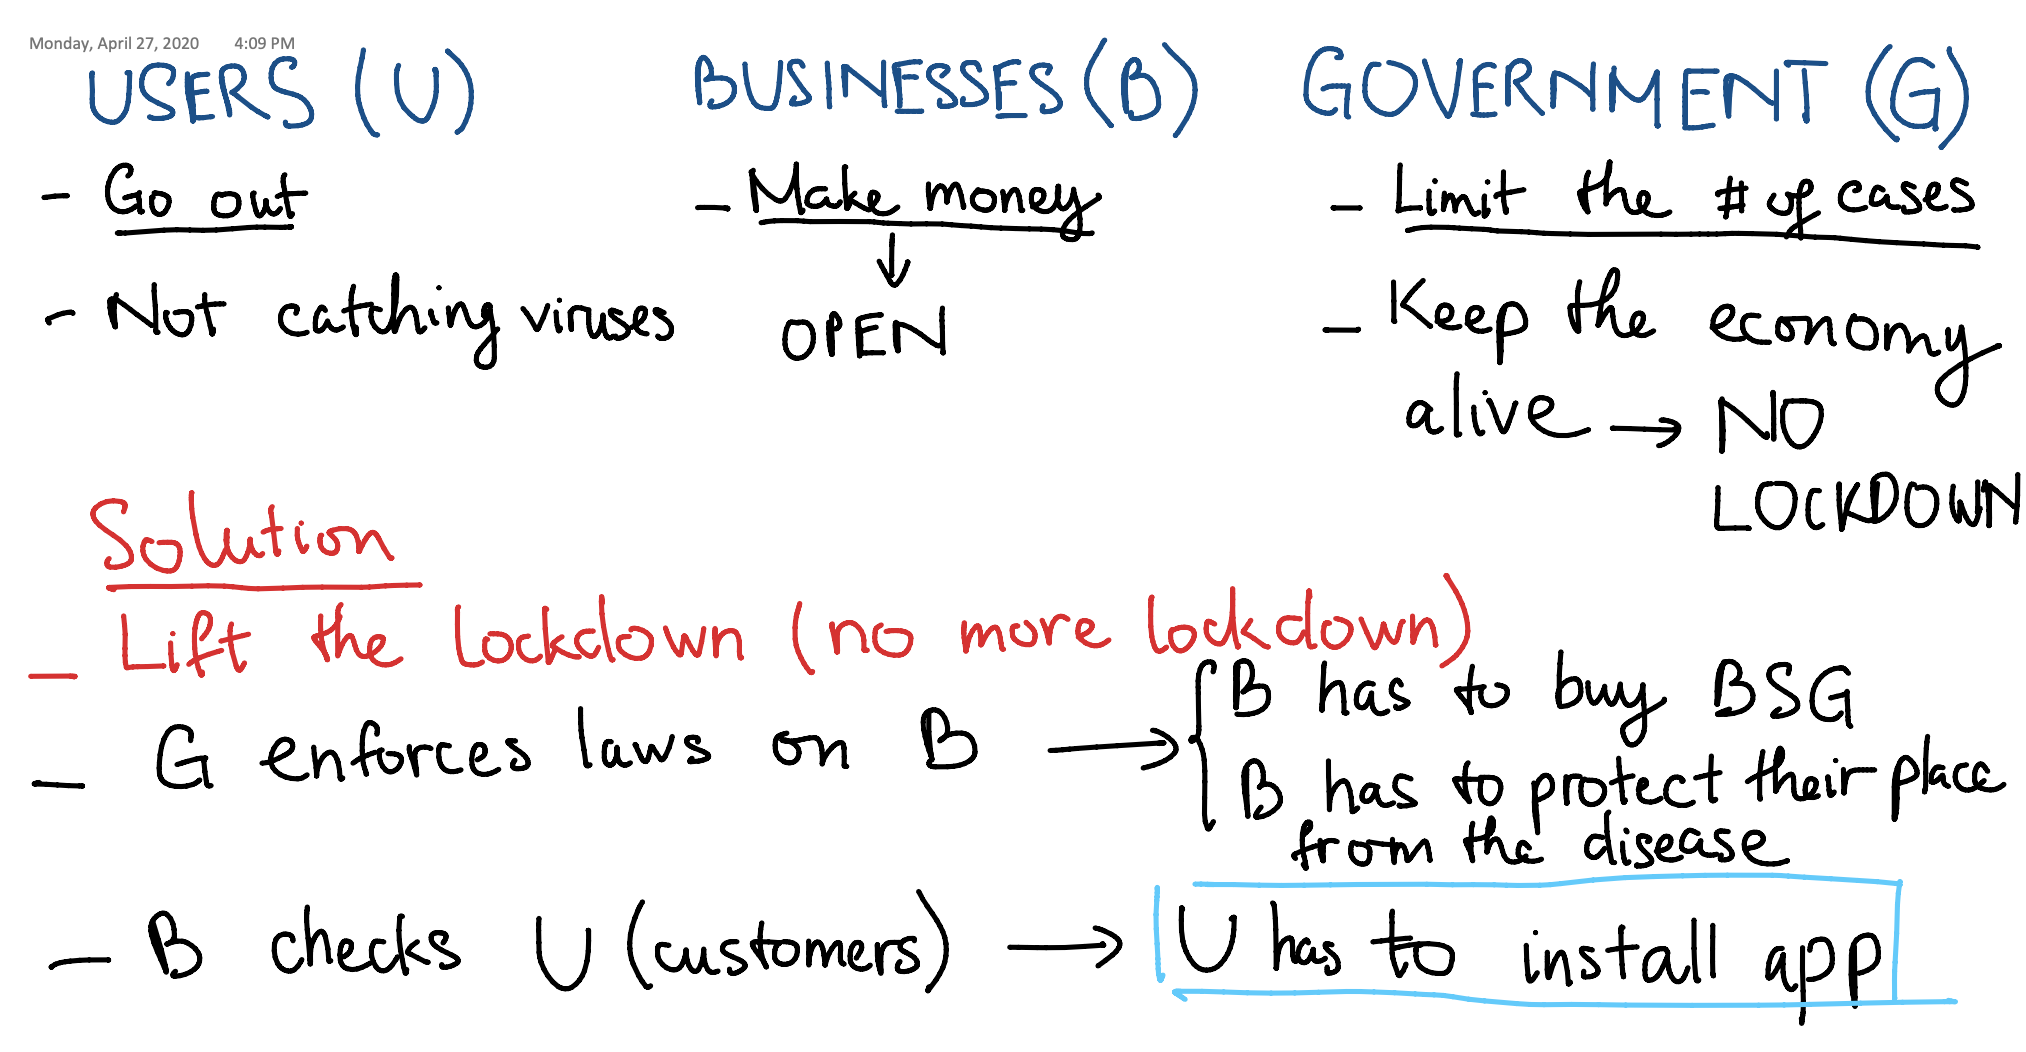
\includegraphics[width=15cm]{solution-model}
    % \caption*{#3}
  \end{figure}

  \par ``BSG'' stands for Bluetooth Signal Generator, which used to be our method of choice for location logging at business until it was found to be impractical to implement. Therefore, we have moved to QR codes as the replacement.

  \subsubsection{Support during lockdown}
  \par Our app, in what other apps have yet to do so, provides different kinds of support for its users throughout the quarantine period:
  \begin{itemize}
    \item The app can be an official channel for people to receive announcements about financial support from the government \parencite{Support5} or care packages from businesses \parencite{Support1}. Users can directly register for these support packages on the app without looking anywhere further.
    \item All emergency/support contacts are listed within the app in terms of which state you are living in \parencite{Support1} \parencite{Support2} \parencite{Support4}. Phone/Online health consultation and medicine prescription are also available. Users can request home-delivered medical supplies from local pharmacies \parencite{Support2}.
    \item The app recommends websites, applications, other online/digital medias which the users can utilize to: \parencite{Support3} \parencite{Support4}
      \begin{itemize}
        \item Keep fit through exercises. Eat and sleep healthily.
        \item Pick up a hobby/Learn new skills: Cooking, Playing musical instruments, Reading, Drawing, Photography, etc.
        \item Get mental advice/support and stay in touch with others.
      \end{itemize} 
  \end{itemize}

  \subsubsection{The technical aspect}
  \par As previously mentioned, our team has changed from Bluetooth Signal Generator (BSG) to QR codes for public places location logging. The reason for this decision was that we discovered it was technically impractical for the BSG to communicate with many devices at the same time. The way Bluetooth communication between devices works is that these devices need to form a connection, also known as pairing with each other, for stable data transmission. Therefore, the BSG would need to keep pairing and unpairing with each device in the area to send them the location code, which becomes near impossible for a large quantity of devices like hundreds or thousands.

